\section{数列的极限}\label{sec:3.2}

\begin{definition}\label{def:3-1}
定义域为正整数的函数称为数列，记为 $\{x_n\}$．即有 $x_n = f(n)$，$n \in \mathbb{N}_+$．
\end{definition}

$x_n$ 是数列的第 $n$ 项，表示函数在 $n$ 处的函数值，而 $\{x_n\}$ 则表示数列．由于正整数有自然的顺序，故数列也可以写成
\[
x_1, x_2, x_3, \cdots, x_n, \cdots.
\]
这也是数列的一种表示．

$x_n$ 也叫做数列的通项，我们经常可以通过给出第 $n$ 项 $x_n$ 的显式来给出一个数列．

例如 $x_n = \frac{1}{n}$，写出来就是 $1, \frac{1}{2}, \frac{1}{3}, \frac{1}{4}, \cdots$；

$x_n = \frac{(-1)^n}{n}$，写出来就是 $-1, \frac{1}{2}, -\frac{1}{3}, \frac{1}{4}, \cdots$；

$x_n = \frac{n+1}{n}$，写出来就是 $2, \frac{3}{2}, \frac{4}{3}, \frac{5}{4}, \cdots$；

$x_n = n^2$，写出来就是 $1, 4, 9, 16, \cdots$；

$x_n = 1+(-1)^n$，写出来就是 $0, 2, 0, 2, \cdots$．

也有些数列的通项不能用显式表示出来．

例如，$c$ 是无理数，它可用无限不循环小数表示
\[
c_0.c_1c_2\cdots c_n\cdots.
\]
令 $x_n = c_0.c_1c_2\cdots c_n$，这样定义的数列 $\{x_n\}$，一般说来，它的通项不能用显式表示出来．

数列也可以用递推的方法给出，例如，$a_0 = 0$，$a_1 = 1$，$a_{n+1} = \frac{a_{n-1}+a_n}{2}$，$n=1,2,\cdots$ 就定义一个数列，它的前六项是
\[
0, 1, \frac{1}{2}, \frac{3}{4}, \frac{5}{8}, \frac{11}{16}.
\]

\subsection*{1. 极限的概念}

根据§\ref{sec:3.1}问题的提出，我们要研究数列的极限，就是看当 $n$ 无限增大时，$x_n$ 的变化趋势如何．换句话说，看是否存在一个常数 $a$，当 $n$ 无限增大时，$x_n$ 的值无限地接近 $a$．在回答是肯定的情形下，就可以说 $\{x_n\}$ 的极限是 $a$．

我们来看前面提出的几个例子．

\begin{example}\label{ex:3-2-1}
$x_n = \frac{1}{n}$．容易看出，当 $n$ 无限增大时，$x_n$ 无限接近于 $0$，因而 $x_n$ 的极限为 $0$．
\end{example}

\begin{example}\label{ex:3-2-2}
$x_n = \frac{(-1)^n}{n}$．当 $n$ 无限增大时，它的值时而为正，时而为负，但总的趋势仍然是无限地接近于 $0$ 这个数，因此 $x_n$ 的极限也是 $0$．
\end{example}

\begin{example}\label{ex:3-2-3}
$x_n = \frac{n+1}{n}$，即
\[
2, \frac{3}{2}, \frac{4}{3}, \frac{5}{4}, \cdots, \frac{101}{100}, \frac{102}{101}, \cdots,
\]
当 $n$ 无限增大时，$x_n$ 越变越小，无限地接近于 $1$，因此 $x_n$ 的极限是 $1$．
\end{example}

\begin{example}\label{ex:3-2-4}
$x_n = n^2$．当 $n$ 无限增大时，$n^2$ 也无限增大，并不无限接近一个常数，因此说它没有极限．
\end{example}

\begin{example}\label{ex:3-2-5}
$x_n = 1+(-1)^n$．它在 $0$ 与 $2$ 两个数中不停地跳动，也不是无限地接近一个常数，因此也没有极限．
\end{example}

现在我们可以来分析一下，一般地说，当 $n$ 无限增大时，$x_n$ 无限接近于 $a$，确切的意思究竟是什么？

两个数接近的程度可以用它们的差的绝对值（在数轴上，就是这两个点之间的距离）来衡量．因此，以 $x_n = \frac{1}{n}$ 为例，说 $x_n$ 与 $0$ 很接近，即是说 $x_n$ 与 $0$ 的距离 $|x_n - 0|$ 很小．例如
\[
\text{当 } n>2 \text{ 时},\quad |x_n - 0| = \frac{1}{n} < \frac{1}{2},
\]
当 $n>3$ 时，$|x_n - 0| = \frac{1}{n} < \frac{1}{3}$，

当 $n>N$ 时，$|x_n - 0| = \frac{1}{n} < \frac{1}{N}$．

上面左边一列是 $n$ 增大的程度．相应地，右边一列是 $x_n$ 与 $0$ 的接近程度．$n$ 增大的程度不同，则 $x_n$ 与 $0$ 的接近程度也不同．$n$ 只要大到比 $N$ 大，就可以保证 $x_n$ 与 $0$ 的距离小于 $\frac{1}{N}$．直观形象地说，如果把数列
\[
x_1, x_2, \cdots, x_N, x_{N+1}, x_{N+2}, \cdots
\]
从第 $N+1$ 项起后面的所有项叫做数列 $\{x_n\}$ 的尾巴，则尾巴中的每项与 $0$ 的距离都小于 $\frac{1}{N}$．

我们已经看到，对于足够大的 $N$ 之后的所有 $n$，可以使 $|x_n - 0|$ 小到一定程度，但还不能说明 $|x_n - 0|$ 无限小．如何反映``无限''二字呢？我们说当 $n$ 无限增大时，$x_n$ 无限接近于 $0$，即是说 $x_n$ 与 $0$ 的距离 $|x_n - 0|$ 可以任意小，只要 $n$ 足够大（$n > N$）．可见``无限''能用距离的任意性来反映，即对于任意的正数 $\varepsilon$，不论它多么小，只要 $N$ 足够大，对于所有的 $n > N$，都能保证 $|x_n - 0| < \varepsilon$．事实上，要使
\[
|x_n - 0| = \frac{1}{n} < \varepsilon,
\]
只要 $n > \frac{1}{\varepsilon}$．故取 $N = \left[\frac{1}{\varepsilon}\right]$，则对大于 $N$ 的所有正整数 $n$，上式总成立．

将上面的语言抽象化，便有下面的定义．

\begin{definition}\label{def:3-2}
设 $\{x_n\}$ 是一数列，$a$ 是一实数．若对于任意给定的正数 $\varepsilon$，存在正整数 $N$，当 $n > N$ 时，都有
\[
|x_n - a| < \varepsilon,
\]
则称 $a$ 是数列 $\{x_n\}$ 当 $n$ 趋于无穷时的极限，或称数列 $\{x_n\}$ 收敛，且收敛于 $a$，记为
\[
\lim_{n\to\infty}x_n = a,\qquad \text{或}\qquad x_n \to a\quad(n\to\infty).
\]
没有极限的数列称为发散数列．
\end{definition}

从几何上看，数列 $\{x_n\}$ 的极限为 $a$，是指任意给定以 $a$ 为中心的区间 $(a-\varepsilon, a+\varepsilon)$，必然从某项 $x_{N+1}$ 起，后面的所有项都落在区间 $(a-\varepsilon, a+\varepsilon)$ 之中．换句话说，数列 $\{x_n\}$ 至多有 $N$ 项 $x_1, x_2, \cdots, x_N$ 落在区间 $(a-\varepsilon, a+\varepsilon)$ 之外（见图~\ref{fig:3-1}）．这就是数列极限的几何意义．由此也可以看出，数列的前有限项并不影响数列的收敛性和极限．即添加或修改数列的有限项，并不影响数列的收敛性与极限．

\begin{figure}[htbp]
\centering
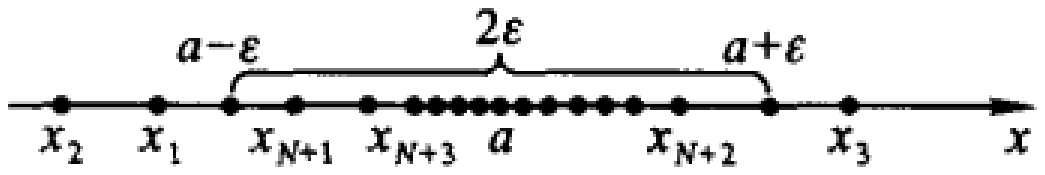
\includegraphics[width=0.72\textwidth]{work/figures/fig3-1}
\figcap\label{fig:3-1}
\end{figure}

定义中描述数列极限的语言称为 $\varepsilon - N$ 语言．正数 $\varepsilon$ 用来反映 $x_n$ 与 $a$ 的接近程度，而 $\varepsilon$ 的任意性就反映了 $x_n$ 与 $a$ 可以任意接近，或说无限接近．$\varepsilon$ 是任意的，也是相对固定的．对每一个固定的 $\varepsilon > 0$，相应地有一个 $N$，$N$ 是随 $\varepsilon$ 的变化而变化的．一般地说，$\varepsilon$ 越小则 $N$ 越大．$N$ 一旦存在则不是唯一的，不过重要的是 $N$ 的存在性，而不是 $N$ 取什么值．

\begin{definition}\label{def:3-3}
极限为 $0$ 的数列称为无穷小量．
\end{definition}

值得注意的是无穷小量是一数列，而不是一个很小的常数．由极限定义显然有，$\{x_n\}$ 以 $a$ 为极限等价于数列 $\{x_n - a\}$ 以 $0$ 为极限．我们把它写成下面的命题．

\begin{proposition}\label{prop:3-1}
$\{x_n\}$ 的极限为 $a$ 的充要条件是 $\{x_n - a\}$ 是无穷小量．
\end{proposition}

数列极限定义本身并没有给出求极限的方法，但它却深刻地描述了数列趋向极限的变化过程．当估计出数列的极限后，可以用定义来验证估计的正确性．下面举例说明．

\begin{example}\label{ex:3-2-6}
证明 $\lim_{n\to\infty}\frac{1}{n^p} = 0$ ($p>0$)．
\end{example}

\begin{proof}
对任意给定的 $\varepsilon>0$，要使
\[
\left|\frac{1}{n^p} - 0\right| = \frac{1}{n^p} < \varepsilon,
\]
只要 $n > \left(\frac{1}{\varepsilon}\right)^{\frac{1}{p}}$．取 $N = \left[\left(\frac{1}{\varepsilon}\right)^{\frac{1}{p}}\right] + 1$，则当 $n > N$ 时，有
\[
\left|\frac{1}{n^p} - 0\right| < \varepsilon.
\]
故 $\left\{\frac{1}{n^p}\right\}$ 的极限为 $0$．
\end{proof}

\begin{example}\label{ex:3-2-7}
设 $|q|<1$，证明 $\lim_{n\to\infty}q^n = 0$．
\end{example}

\begin{proof}[证法 1]
若 $q = 0$，结论显然成立．故不妨设 $q \neq 0$．对任意给定的 $\varepsilon > 0$，不妨设 $\varepsilon < 1$，要使
\[
|q^n - 0| = |q^n| < \varepsilon,
\]
即
\[
n\lg|q| < \lg\varepsilon,
\]
只要
\[
n > \frac{\lg\varepsilon}{\lg|q|}.
\]
令 $N = \left[\frac{\lg\varepsilon}{\lg|q|}\right] + 1$，则当 $n > N$ 时，有 $|q^n| < \varepsilon$．这就证明了 $\lim_{n \to \infty} q^n = 0$．
\end{proof}

\begin{proof}[证法 2]
不妨设 $q \neq 0$．由 $|q| < 1$ 知存在 $\alpha > 0$，使得 $|q| = \frac{1}{1 + \alpha}$，从而
\[
|q|^n = \frac{1}{(1 + \alpha)^n} = \frac{1}{1 + n\alpha + \cdots + \alpha^n} < \frac{1}{n\alpha}.
\]
对任给的 $\varepsilon > 0$，要使 $|q^n| < \varepsilon$，只要放大后的 $\frac{1}{n\alpha} < \varepsilon$．因此取 $N = \left[\frac{1}{\alpha\varepsilon}\right] + 1$，则当 $n > N$ 时，有
\[
|q^n - 0| = |q|^n < \frac{1}{n\alpha} < \varepsilon.
\]
这就证明了 $\lim_{n\to\infty}q^n = 0$．
\end{proof}

从前面的例子可见，整个证明过程实际上是找 $N$ 的过程，采用的是反推法，即从 $|x_n - a| < \varepsilon$ 出发，看满足条件的 $N$ 是否存在．我们只要找到一个就可以了，不管用的是什么方法．证法 2 用的是适当放大法，它将 $|q^n - 0|$ 适当放大到 $\frac{1}{n\alpha}$，使我们很容易找到 $N$．当然放大要适当，要保证把 $|x_n - a|$ 放大以后仍然是无穷小量．下面再举几个适当放大的例子．

\begin{example}\label{ex:3-2-8}
设 $a > 0$，证明 $\lim_{n \to \infty} \sqrt[n]{a} = 1$．
\end{example}

\begin{proof}
若 $a=1$，结论显然成立．

设 $a > 1$．记 $\sqrt[n]{a} = 1 + \alpha_n$ ($\alpha_n > 0$)，则
\[
a = (1 + \alpha_n)^n = 1 + n\alpha_n + \cdots + \alpha_n^n > n\alpha_n.
\]
因此
\[
|\sqrt[n]{a} - 1| = \alpha_n < \frac{a}{n}.
\]
对任意给定的 $\varepsilon>0$，不妨设 $\varepsilon<1$，取 $N = \left[\frac{a}{\varepsilon}\right]$，则当 $n>N$ 时，有
\[
|\sqrt[n]{a} - 1| < \frac{a}{n} < \varepsilon.
\]
最后设 $0 < a < 1$．这时存在 $b > 1$ 使 $a = \frac{1}{b}$，因此
\[
|\sqrt[n]{a} - 1| = \left|\sqrt[n]{\frac{1}{b}} - 1\right| = \frac{|1 - \sqrt[n]{b}|}{\sqrt[n]{b}} < |1 - \sqrt[n]{b}|.
\]
由于 $\lim_{n\to\infty}\sqrt[n]{b} = 1$，故对任给 $\varepsilon>0$，存在 $N$，当 $n>N$ 时，有
\[
|\sqrt[n]{a} - 1| < |1 - \sqrt[n]{b}| < \varepsilon.
\]
这样，我们证明了当 $a > 0$ 时，总有 $\lim_{n \to \infty} \sqrt[n]{a} = 1$．
\end{proof}

\begin{example}\label{ex:3-2-9}
证明 $\lim_{n\to\infty}\frac{n^2+1}{n^2-n-2} = 1$．
\end{example}

\begin{proof}
当 $n>4$ 时，
\[
\left|\frac{n^2+1}{n^2-n-2} - 1\right| = \left|\frac{n+3}{n^2-n-2}\right| = \frac{n+3}{n^2-n-2} < \frac{2n}{n^2 - \frac{n^2}{4} - \frac{n^2}{4}} = \frac{4}{n}.
\]
对任给的 $\varepsilon>0$，取 $N = \max\left(4, \left[\frac{4}{\varepsilon}\right]\right)$，则当 $n>N$ 时，有
\[
\left|\frac{n^2+1}{n^2-n-2} - 1\right| < \frac{4}{n} < \varepsilon,
\]
即
\[
\lim_{n\to\infty}\frac{n^2+1}{n^2-n-2} = 1.
\]
\end{proof}

研究数列的极限，就是要从数列出发，把它的极限求出来．可见从数列到极限，也是一种运算，但它同第一章讲数系时的运算很不同．那时是从两个数（或有穷个数）出发求一个数，例如从 $a$ 和 $b$ 求 $a+b$．求极限则完全不同了，是从一个数列，即从无穷个数出发，求一个数．从无穷个数到一个数，这就是极限运算的特点．正是由于这个特点，使极限的计算变得十分复杂．因此，人们需要有一个一般的准则来检验计算是否正确．当然，这个准则不仅在检验一些具体数列的极限时是重要的，而更重要的是它对理论上的推理是必不可少的．这个准则就是极限的 $\varepsilon-N$ 定义，它是人类经过漫长的时间才抽象出来的．我们并不要求读者立刻全面地理解，只希望读者在今后的学习过程中，通过大量的反复的应用逐步地掌握它．

\subsection*{2. 极限与四则运算及与不等式的关系}

下面我们要来寻找求极限的方法．

回忆学算术的过程，我们可以计算任何两个数的乘法．为什么呢？实际上，我们所掌握的，一是九九表，二是一套进位规则（当然还包括小数点的计算）．何谓进位规则？其实说的是加法与乘法的分配律，也就是加法与乘法的运算次序可以交换：
\[
a(b+c) = ab + ac.
\]
例如，$26 \times 8 = 208$，是这样计算出来的：
\[
\begin{array}{r}
2\ 6 \\
\times \quad 8 \\
\hline
4\ 8 \\
1\ 6\ 0 \\
\hline
2\ 0\ 8
\end{array}
\]
实际上根据的就是加法与乘法可以交换次序：
\[
26\times8 = (20+6)\times8 = 20\times8 + 6\times8 = 160 + 48 = 208.
\]
因此，我们希望能学会求更多数列的极限，自然就会问，对极限这一新的运算，它和别的运算间是否也有类似的规律？事实上，并非所有的运算都具有类似的性质．例如等式
\[
\sqrt{a+b} = \sqrt{a} + \sqrt{b}
\]
就不是永远成立的，即开平方运算与加法运算并不能交换次序．若能设想这等式成立，开平方运算就会变得简单得多了．

极限是对无穷个数进行的运算，它和四则运算的次序能否交换？幸好，回答是肯定的．当然，这是需要证明的，因为极限运算是一种崭新的运算．

\begin{theorem}\label{thm:3-1}
设 $\lim_{n\to\infty}x_n = a$，$\lim_{n\to\infty}y_n = b$，则
\begin{enumerate}[label=\roman*)]
\item $\lim_{n\to\infty}(x_n \pm y_n) = a \pm b$；
\item $\lim_{n \to \infty} (x_n y_n) = ab$；
\item $\lim_{n \to \infty} \frac{x_n}{y_n} = \frac{a}{b} \quad (b \neq 0)$．
\end{enumerate}
\end{theorem}

定理~\ref{thm:3-1} 表明两数列对应项的代数和（积、商）的极限等于极限的代数和（积、商），因此实际上说的是极限运算和四则运算次序是可以交换的．我们可以把定理~\ref{thm:3-1} 写成
\[
\lim_{n\to\infty}(x_n \pm y_n) = \lim_{n\to\infty}x_n \pm \lim_{n\to\infty}y_n;
\]
\[
\lim_{n\to\infty}(x_n y_n) = \lim_{n\to\infty}x_n \cdot \lim_{n\to\infty}y_n;
\]
\[
\lim_{n\to\infty}\frac{x_n}{y_n} = \frac{\lim\limits_{n\to\infty}x_n}{\lim\limits_{n\to\infty}y_n}\qquad \left(\text{当 }\lim_{n\to\infty}y_n \neq 0\right).
\]
值得注意的是，其前提是等式右边的极限都事先假设是存在的．

为了证明 ii)，我们将要用到收敛数列的有界性．为了证明 iii)，又要用到极限的保号性．因此，我们先给出这两个性质，再回头来证明定理~\ref{thm:3-1}．

回忆函数的有界性定义，知数列 $\{x_n\}$ 有界是指存在正数 $M$，使得
\[
|x_n| \leqslant M
\]
对一切 $n$ 成立．

\begin{theorem}[有界性]\label{thm:3-2}
有极限存在的数列必有界．
\end{theorem}

\begin{proof}
设数列 $\{x_n\}$ 有极限 $a$．由极限定义，对 $\varepsilon_0 = 1$，则存在 $N$，当 $n>N$ 时，有
\[
|x_n - a| < 1.
\]
因此
\[
|x_n| = |x_n - a + a| \leqslant |x_n - a| + |a| < 1 + |a|.
\]
令 $M = \max(|x_1|, |x_2|, \cdots, |x_N|, 1+|a|)$，则
\[
|x_n| \leqslant M,\qquad n=1,2,\cdots.
\]
这就证明了 $\{x_n\}$ 是有界的．
\end{proof}

\begin{corollary}\label{cor:3-1}
若 $\{x_n\}$ 无界，则 $\{x_n\}$ 发散．
\end{corollary}

\begin{theorem}[保号性]\label{thm:3-3}
若 $\lim_{n\to\infty}x_n = a$，$a>0$，则存在 $N$，当 $n>N$ 时，有 $x_n > \frac{a}{2} > 0$．
\end{theorem}

\begin{proof}
由 $\lim_{n\to\infty}x_n = a > 0$，知对 $\varepsilon_0 = \frac{a}{2} > 0$，存在 $N$，当 $n>N$ 时，有
\[
|x_n - a| < \frac{a}{2},
\]
从而
\[
x_n > a - \frac{a}{2} = \frac{a}{2} > 0.
\]
定理证完（见图~\ref{fig:3-2}）．
\end{proof}

\begin{figure}[htbp]
\centering
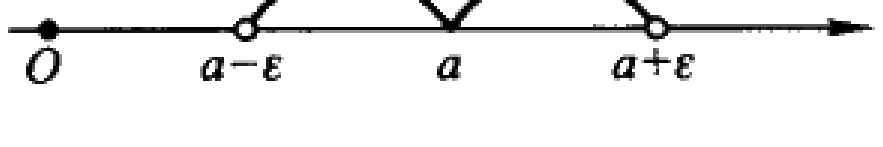
\includegraphics[width=0.48\textwidth]{work/figures/fig3-2}
\figcap\label{fig:3-2}
\end{figure}

\begin{corollary}\label{cor:3-2}
设 $\lim_{n\to\infty}x_n = a$．
\begin{enumerate}[label=\roman*)]
\item 若 $a<0$，则存在 $N$，当 $n>N$ 时，有 $x_n < \frac{a}{2} < 0$；
\item 若 $a \neq 0$，则存在 $N$，当 $n > N$ 时，有 $|x_n| > \frac{|a|}{2} > 0$．
\end{enumerate}
\end{corollary}

请读者写出推论~\ref{cor:3-2} 的证明．

\begin{proof}[定理~\ref{thm:3-1} 的证明]
i) 对任意给定的 $\varepsilon>0$，由 $\lim_{n\to\infty} x_n = a$，存在 $N_1$，当 $n>N_1$ 时，有
\[
|x_n - a| < \frac{\varepsilon}{2}.
\]
由 $\lim_{n\to\infty}y_n = b$，知存在 $N_2$，当 $n>N_2$ 时，有
\[
|y_n - b| < \frac{\varepsilon}{2}.
\]
取 $N = \max(N_1, N_2)$，则当 $n > N$ 时，有
\[
|x_n \pm y_n - (a \pm b)| \leqslant |x_n - a| + |y_n - b| < \frac{\varepsilon}{2} + \frac{\varepsilon}{2} = \varepsilon,
\]
即
\[
\lim_{n\to\infty}(x_n \pm y_n) = a \pm b.
\]

ii) 对任意 $n$，有
\[
\begin{aligned}
|x_n y_n - ab| &= |x_n y_n - x_n b + x_n b - ab| \\
&\leqslant |x_n y_n - x_n b| + |x_n b - ab| \\
&= |x_n||y_n - b| + |b||x_n - a|.
\end{aligned}
\]
任给 $\varepsilon>0$，由 $\lim_{n\to\infty}x_n = a$ 与 $\lim_{n\to\infty}y_n = b$，以及定理~\ref{thm:3-2}，知存在 $M>0$，使
\[
|x_n| \leqslant M,\qquad n=1,2,\cdots,
\]
同时存在 $N_1$，当 $n > N_1$ 时，有
\[
|x_n - a| < \frac{\varepsilon}{2(|b|+1)},
\]
并存在 $N_2$，当 $n > N_2$ 时，有
\[
|y_n - b| < \frac{\varepsilon}{2M}.
\]
令 $N = \max(N_1, N_2)$，则当 $n > N$ 时，有
\[
|x_n y_n - ab| \leqslant |x_n||y_n - b| + |b||x_n - a| < M\frac{\varepsilon}{2M} + |b|\frac{\varepsilon}{2(|b|+1)} < \varepsilon.
\]
这就证明了 $\lim_{n\to\infty}x_n y_n = ab$．

iii) 由 $\lim_{n\to\infty}y_n = b \neq 0$，根据推论~\ref{cor:3-2}，存在 $N_1$，当 $n>N_1$ 时，有
\[
|y_n| > \frac{|b|}{2} > 0,
\]
从而当 $n>N_1$ 时有
\[
\left|\frac{x_n}{y_n} - \frac{a}{b}\right| = \frac{|b x_n - a y_n|}{|y_n||b|} \leqslant \frac{|b||x_n - a| + |a||y_n - b|}{\frac{1}{2}|b|^2}.
\]
已知 $\lim_{n\to\infty}x_n = a$ 和 $\lim_{n\to\infty}y_n = b$，由极限定义，对任意给定的 $\varepsilon>0$，存在 $N_2$，当 $n>N_2$ 时，有
\[
|x_n - a| < \frac{|b|}{4}\varepsilon,
\]
存在 $N_3$，当 $n > N_3$ 时，有
\[
|y_n - b| < \frac{|b|^2}{4(|a|+1)}\varepsilon.
\]
令 $N = \max(N_1, N_2, N_3)$，则当 $n > N$ 时，有
\[
\left|\frac{x_n}{y_n} - \frac{a}{b}\right| \leqslant \frac{2}{|b|}|x_n - a| + \frac{2|a|}{|b|^2}|y_n - b| < \frac{\varepsilon}{2} + \frac{\varepsilon}{2} = \varepsilon.
\]
这就证明了 $\lim_{n\to\infty}\frac{x_n}{y_n} = \frac{a}{b}$．
\end{proof}

当 $x_n = c$ 时，我们由 ii) 得到下面的推论．

\begin{corollary}\label{cor:3-3}
若 $\lim_{n\to\infty}y_n = b$，$c$ 是常数，则
\[
\lim_{n\to\infty}(c y_n) = cb.
\]
\end{corollary}

在定理~\ref{thm:3-2} 和定理~\ref{thm:3-3} 的证明中，$\varepsilon$ 不是任意的，而是取定了某 $\varepsilon_0$，$\varepsilon_0$ 不变才能保证 $N$ 固定不变．而在定理~\ref{thm:3-1} 的证明中 $\varepsilon$ 都是任意的．请注意区别什么时候可以取定 $\varepsilon$，而什么时候 $\varepsilon$ 必须是任意的．

由定理~\ref{thm:3-1} 的 i) 以及 ii) 立即可知，无穷小量的代数和、积仍是无穷小量．对于积，我们还有下面的结论，它对求极限是很方便的．

\begin{theorem}\label{thm:3-4}
若 $\{x_n\}$ 是无穷小量，$\{y_n\}$ 是有界数列，则 $\{x_n y_n\}$ 是无穷小量．
\end{theorem}

\begin{proof}
对任意给定的 $\varepsilon>0$，首先由 $\{y_n\}$ 是有界数列，知存在 $M>0$，使得
\[
|y_n| \leqslant M,\qquad n=1,2,\cdots.
\]
其次由 $\{x_n\}$ 是无穷小量，知存在 $N$，当 $n > N$ 时，有
\[
|x_n| < \frac{\varepsilon}{M}.
\]
因此，当 $n > N$ 时，有
\[
|x_n y_n| \leqslant M|x_n| < \varepsilon.
\]
定理证完．
\end{proof}

\begin{example}\label{ex:3-2-10}
求 $\lim_{n\to\infty}\frac{1}{n}\sin n$．
\end{example}

\begin{proof}[解]
因为 $\lim_{n\to\infty}\frac{1}{n} = 0$，而 $\{\sin n\}$ 是有界数列，所以
\[
\lim_{n\to\infty}\frac{1}{n}\sin n = 0.
\]
\end{proof}

\begin{example}\label{ex:3-2-11}
求 $\lim_{n\to\infty}\frac{4n^2+1}{2n^2+5n-6}$．
\end{example}

\begin{proof}[解]
\[
\lim_{n\to\infty}\frac{4n^2+1}{2n^2+5n-6} = \lim_{n\to\infty}\frac{4+\frac{1}{n^2}}{2+\frac{5}{n}-\frac{6}{n^2}} = \frac{4+\lim\limits_{n\to\infty}\frac{1}{n^2}}{2+\lim\limits_{n\to\infty}\frac{5}{n}-\lim\limits_{n\to\infty}\frac{6}{n^2}} = 2.
\]
\end{proof}

更一般地，若 $a_0 \neq 0$，$b_0 \neq 0$，$k,l$ 是正整数，$k \leqslant l$，则
\[
\lim_{n\to\infty}\frac{a_0 n^k + a_1 n^{k-1} + \cdots + a_k}{b_0 n^l + b_1 n^{l-1} + \cdots + b_l} = \lim_{n\to\infty}n^{k-l}\frac{a_0 + \frac{a_1}{n} + \cdots + \frac{a_k}{n^k}}{b_0 + \frac{b_1}{n} + \cdots + \frac{b_l}{n^l}} = \begin{cases}
\frac{a_0}{b_0}, & k = l,\\
0, & k < l.
\end{cases}
\]

下面研究极限运算与不等式的关系．

\begin{theorem}[保序性]\label{thm:3-5}
若 $\lim_{n\to\infty}x_n = a$，$\lim_{n\to\infty}y_n = b$，且 $a>b$，则存在 $N$，当 $n>N$ 时，有 $x_n > y_n$．
\end{theorem}

\begin{proof}[证法 1]
（用定理~\ref{thm:3-3} 的证明方法）对 $\varepsilon_0 = \frac{a-b}{2}$，由 $\lim_{n\to\infty}x_n = a$，知存在 $N_1$，当 $n>N_1$ 时，有
\[
|x_n - a| < \frac{a-b}{2},
\]
则有
\[
\frac{a+b}{2} < x_n.
\]
又由 $\lim_{n\to\infty}y_n = b$，知存在 $N_2$，当 $n>N_2$ 时，有
\[
|y_n - b| < \frac{a-b}{2},
\]
则有
\[
y_n < \frac{a+b}{2}.
\]
令 $N = \max(N_1, N_2)$，则当 $n > N$ 时，有
\[
y_n < \frac{a+b}{2} < x_n.
\]
定理证完（见图~\ref{fig:3-3}）．
\end{proof}

\begin{figure}[htbp]
\centering
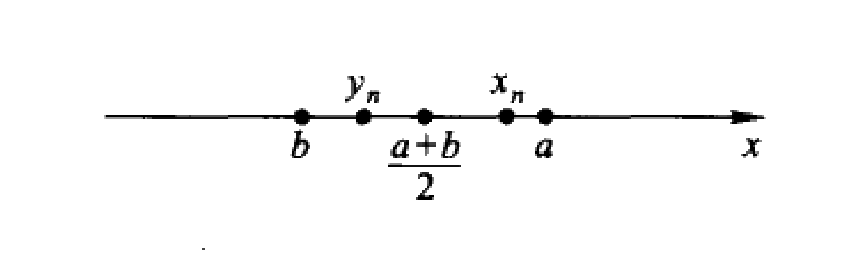
\includegraphics[width=0.55\textwidth]{work/figures/fig3-3}
\figcap\label{fig:3-3}
\end{figure}

\begin{proof}[证法 2]
令 $z_n = x_n - y_n$，则
\[
\lim_{n\to\infty}z_n = \lim_{n\to\infty}(x_n - y_n) = a - b > 0.
\]
由定理~\ref{thm:3-3}，存在 $N$，当 $n > N$ 时，有
\[
z_n = x_n - y_n > \frac{a-b}{2} > 0,
\]
即 $x_n > y_n$．这又证明了定理~\ref{thm:3-5}．
\end{proof}

值得指出的是，证法 1 用的是定理~\ref{thm:3-3} 的证明方法，证法 2 用的是定理~\ref{thm:3-3} 的结论．用定理的结论，和用定理的证明方法，是不同的两回事．对一个定理，既要学会用它的结论，也要学会用它的证明方法，这是以后学习要注意的．

\begin{theorem}[极限不等式]\label{thm:3-6}
若对任意正整数 $n$ 有 $x_n \leqslant y_n$，且 $\lim_{n \to \infty} x_n = a$，$\lim_{n \to \infty} y_n = b$，则 $a \leqslant b$．
\end{theorem}

\begin{proof}
用反证法．如果不然，设 $a > b$，则由定理~\ref{thm:3-5}，存在 $N$，当 $n > N$ 时有 $x_n > y_n$，与假设条件矛盾．故必有 $a \leqslant b$．
\end{proof}

注意到数列的前有限项并不影响数列的极限，因此定理~\ref{thm:3-6} 的条件可以减弱为``存在 $N$，当 $n > N$ 时有 $x_n \leqslant y_n$''．

如果将条件``$x_n \leqslant y_n$''改为``$x_n < y_n$''，并不能得到 $a < b$ 的结论．例如 $\frac{n-1}{n} < \frac{n+1}{n}$，但
\[
\lim_{n\to\infty}\frac{n-1}{n} = \lim_{n\to\infty}\frac{n+1}{n} = 1.
\]
可见结论也只能得到 $a \leqslant b$．定理~\ref{thm:3-6} 表明，在极限存在的前提下，可以在不等式两边取极限，但千万不要忘记``带上等号''．

用上面的方法，我们实际上已证明了极限的唯一性，即一个数列不可能有两个不同的极限值．

\begin{theorem}[唯一性]\label{thm:3-7}
若数列有极限存在，则极限是唯一的．
\end{theorem}

\begin{proof}
用反证法．如果不然，设 $\{x_n\}$ 有极限 $a$ 和 $b$，$a \neq b$，不妨设 $a < b$．对 $\varepsilon = \frac{b - a}{2} > 0$，存在 $N_1$，当 $n > N_1$ 时，有
\[
x_n < a + \varepsilon = \frac{a+b}{2},
\]
同样存在 $N_2$，当 $n > N_2$ 时，有
\[
x_n > b - \varepsilon = \frac{a+b}{2},
\]
故当 $n > \max (N_1, N_2)$ 时，有
\[
x_n < a + \varepsilon = b - \varepsilon = \frac{a+b}{2} < x_n,
\]
这是不可能的，这就证明了极限的唯一性．
\end{proof}

\begin{theorem}[夹迫性]\label{thm:3-8}
如果对任意正整数 $n$，有
\[
x_n \leqslant y_n \leqslant z_n,
\]
且 $\lim_{n\to\infty}x_n = \lim_{n\to\infty}z_n = a$，则 $\lim_{n\to\infty}y_n$ 存在且等于 $a$．
\end{theorem}

\begin{proof}
对任意给定的 $\varepsilon > 0$，由 $\lim_{n \to \infty} x_n = \lim_{n \to \infty} z_n = a$，存在 $N_1$，当 $n > N_1$ 时，有
\[
|x_n - a| < \varepsilon,\qquad \text{即}\quad a-\varepsilon < x_n < a+\varepsilon.
\]
存在 $N_2$，当 $n > N_2$ 时，有
\[
|z_n - a| < \varepsilon,\qquad \text{即}\quad a-\varepsilon < z_n < a+\varepsilon.
\]
令 $N = \max(N_1, N_2)$，则当 $n > N$ 时，有
\[
a-\varepsilon < x_n \leqslant y_n \leqslant z_n < a+\varepsilon,
\]
即
\[
|y_n - a| < \varepsilon.
\]
故 $\lim_{n\to\infty}y_n$ 存在且等于 $a$，定理证完．
\end{proof}

\begin{example}\label{ex:3-2-12}
设 $x_n = \sqrt[n]{A^n + B^n}$，其中 $A>B>0$，求证 $\lim_{n\to\infty}x_n = A$．
\end{example}

\begin{proof}
由于
\[
A = \sqrt[n]{A^n} \leqslant \sqrt[n]{A^n + B^n} \leqslant \sqrt[n]{2A^n} = \sqrt[n]{2}A,
\]
而
\[
\lim_{n\to\infty}\sqrt[n]{2}A = 1\cdot A = A,
\]
由定理~\ref{thm:3-8} 即得 $\lim_{n\to\infty}\sqrt[n]{A^n + B^n} = A$．
\end{proof}

\begin{example}\label{ex:3-2-13}
证明 $\lim_{n\to\infty}\sqrt[n]{n} = 1$．
\end{example}

\begin{proof}[证法 1]
当 $n > 1$ 时，$\sqrt[n]{n} > 1$，令 $\sqrt[n]{n} = 1 + h_n$，其中 $h_n > 0$．这时
\[
n = (1+h_n)^n = 1 + nh_n + \frac{n(n-1)}{2}h_n^2 + \cdots + h_n^n \geqslant \frac{n(n-1)}{2}h_n^2,
\]
因此 $h_n \leqslant \sqrt{\frac{2}{n-1}}$．故
\[
1 < \sqrt[n]{n} = 1 + h_n \leqslant 1 + \sqrt{\frac{2}{n-1}}.
\]
已知
\[
\lim_{n\to\infty}\left(1 + \sqrt{\frac{2}{n-1}}\right) = 1 + \lim_{n\to\infty}\sqrt{\frac{2}{n-1}} = 1,
\]
由定理~\ref{thm:3-8} 得 $\lim_{n\to\infty}\sqrt[n]{n} = 1$．
\end{proof}

\begin{proof}[证法 2]
当 $n>1$ 时，由平均值不等式得
\[
1 < \sqrt[n]{n} = \sqrt[n]{\sqrt{n}\cdot\sqrt{n}\cdot1\cdots1} \leqslant \frac{\sqrt{n} + \sqrt{n} + n - 2}{n} = \frac{2}{\sqrt{n}} + 1 - \frac{2}{n}.
\]
而
\[
\lim_{n\to\infty}\left(\frac{2}{\sqrt{n}} + 1 - \frac{2}{n}\right) = 1,
\]
由定理~\ref{thm:3-8} 得 $\lim_{n\to\infty}\sqrt[n]{n} = 1$．
\end{proof}

回忆函数单调性定义，我们说数列 $\{x_n\}$ 单调上升（下降），是指 $x_n \leqslant x_{n+1}$（$x_n \geqslant x_{n+1}$）对一切 $n$ 成立．

\begin{theorem}\label{thm:3-9}
单调上升（下降）有上（下）界的数列必有极限存在．
\end{theorem}

\begin{proof}
设数列 $\{x_n\}$ 单调上升有上界．令 $B$ 是 $\{x_n\}$ 全体上界组成的集合，即
\[
B = \{b\mid x_n \leqslant b,\,\forall n\},
\]
而
\[
A = \mathbb{R}\setminus B,
\]
则 $A \mid B$ 是实数的一个分划．事实上，由 $\{x_n\}$ 有上界，知 $B$ 不空．又 $\{x_n\}$ 单调上升，故 $x_1 - 1 \in A$，即 $A$ 不空．由 $A = \mathbb{R} \setminus B$ 知，$A,B$ 不漏．又对任给 $a \in A, b \in B$，则存在 $n_0$，使 $a < x_{n_0} \leqslant b$，即 $A,B$ 不乱．故 $A \mid B$ 是实数的一个分划．根据实数基本定理，存在 $\alpha \in \mathbb{R}$ 使得对任意 $a \in A$，任意 $b \in B$，有 $a \leqslant \alpha \leqslant b$．

下证 $\lim_{n\to\infty}x_n = \alpha$．事实上，对任给 $\varepsilon>0$，由于 $\alpha-\varepsilon \in A$，知存在 $N$，使 $\alpha-\varepsilon < x_N$，又 $\{x_n\}$ 单调上升，故当 $n>N$ 时，有 $\alpha-\varepsilon < x_N \leqslant x_n$．注意到 $\alpha+\frac{\varepsilon}{2} \in B$，便有 $x_n \leqslant \alpha+\frac{\varepsilon}{2}$，故当 $n>N$ 时有
\[
\alpha-\varepsilon < x_n \leqslant \alpha+\frac{\varepsilon}{2},
\]
于是
\[
|x_n - \alpha| < \varepsilon.
\]
这就证明了 $\lim_{n\to\infty}x_n = \alpha$．

显然，单调下降的情形同样可以用上述证明方法给出，但也可以用上述结论证明．事实上，若 $\{x_n\}$ 单调下降有下界，令 $y_n = -x_n$，则 $\{y_n\}$ 就单调上升有上界，从而有极限．设极限为 $\alpha$，则
\[
\lim_{n\to\infty}x_n = \lim_{n\to\infty}(-y_n) = -\lim_{n\to\infty}y_n = -\alpha.
\]
定理证完．
\end{proof}

定理~\ref{thm:3-9} 是只断言极限存在，而没有给出如何计算极限的第一个定理．但即使只给出极限存在，有时已能提供计算的方法．

\begin{example}\label{ex:3-2-14}
设
\[
\begin{aligned}
&x_1 = \sqrt{2},\quad x_2 = \sqrt{2+\sqrt{2}},\\
&x_{n+1} = \sqrt{2+x_n} = \sqrt{2+\sqrt{2+\cdots+\sqrt{2}}},\qquad n=2,3,\cdots,
\end{aligned}
\]
求 $\{x_n\}$ 的极限．
\end{example}

\begin{proof}[解]
显然 $\{x_n\}$ 是单调上升的，下面用数学归纳法证明 $\{x_n\}$ 有上界．显然 $x_1 = \sqrt{2} < 2$．若 $x_n \leqslant 2$，则
\[
x_{n+1} = \sqrt{2+x_n} \leqslant \sqrt{2+2} = 2.
\]
故 $\{x_n\}$ 单调上升有上界，从而必有极限．设极限为 $a$，由
\[
x_{n+1}^2 = 2 + x_n,
\]
令 $n \to \infty$，即得 $a^2 = 2 + a$．解得 $a = -1$ 或 $a = 2$．由于 $x_n \geqslant \sqrt{2}$，故必有 $a \geqslant \sqrt{2}$．舍去 $a = -1$，得 $a = 2$，即 $\lim_{n \to \infty} x_n = 2$．
\end{proof}

通常我们称定理~\ref{thm:3-9} 为单调有界原理，它的意义在于给出了数列极限存在的一个判别方法．与极限定义相比，它并不需要预先估计极限值，相反，如上例表明的，有时在用它证明了极限存在的情况下，通过极限的运算可以方便地求出极限值．但务必注意，在这里极限存在性的前提是非常重要的．考察数列 $x_n = (-1)^n$，显然 $\{x_n\}$ 的极限不存在（本节习题 10），但它满足 $x_{n+1} = -x_n$．令 $n\to\infty$ 两边取极限，便得 $a = -a$，即 $a = 0$．这显然是荒谬的结果．

最后，我们用单调有界原理证明一个重要数列极限的存在性．

\begin{example}\label{ex:3-2-15}
证明数列 $\left\{\left(1+\frac{1}{n}\right)^n\right\}$ 的极限存在．
\end{example}

\begin{proof}
先证 $\left\{\left(1+\frac{1}{n}\right)^n\right\}$ 是单调上升的，即证
\[
\left(1+\frac{1}{n}\right)^n \leqslant \left(1+\frac{1}{n+1}\right)^{n+1},
\]
或
\[
\sqrt[n+1]{\left(1+\frac{1}{n}\right)^n} \leqslant 1 + \frac{1}{n+1}.
\]
由平均值不等式即得
\[
\sqrt[n+1]{\left(1+\frac{1}{n}\right)^n\cdot 1} \leqslant \frac{n\left(1+\frac{1}{n}\right) + 1}{n+1} = 1 + \frac{1}{n+1}.
\]
再证 $\left\{\left(1+\frac{1}{n}\right)^n\right\}$ 有上界．我们试图证明 $\left(1+\frac{1}{n}\right)^n < 4$．即要证
\[
\sqrt[n]{\frac{1}{4}} < \frac{n}{n+1}.
\]
此式当 $n=1$ 时显然成立，当 $n>1$ 时，由平均值不等式即得
\[
\sqrt[n]{\frac{1}{4}} = \sqrt[n]{\frac{1}{2}\cdot\frac{1}{2}\cdot1\cdots1} \leqslant \frac{\frac{1}{2} + \frac{1}{2} + (n-2)}{n} = 1 - \frac{1}{n} < 1 - \frac{1}{n+1} = \frac{n}{n+1}.
\]
故由单调有界原理知 $\lim_{n\to\infty}\left(1+\frac{1}{n}\right)^n$ 存在．
\end{proof}

通常我们记这个极限为 $\mathrm{e}$，它是一个无理数，用前几位小数表示即为
\[
\lim_{n\to\infty}\left(1+\frac{1}{n}\right)^n = \mathrm{e} = 2.718\,281\,8\cdots.
\]
称以 $\mathrm{e}$ 为底的对数为自然对数，记为 $\log_{\mathrm{e}}x = \ln x$．为什么称这是``自然对数''，读者学到后面便会明白．

\subsection*{3. 无穷大量}

在发散的数列中有一种特殊的数列，就是当 $n$ 无限增大时，$|x_n|$ 也无限增大，例如 $\{n^2\}$ 和 $\{(-2)^n\}$．我们称这种数列为无穷大量．仿照数列极限的 $\varepsilon-N$ 语言，我们给出无穷大量的严格定义．

\begin{definition}\label{def:3-4}
设 $\{x_n\}$ 是一数列．若对于任意给定的 $G > 0$，存在正整数 $N$，当 $n > N$ 时，有 $|x_n| > G$，则称 $\{x_n\}$ 是无穷大量，记为
\[
\lim_{n\to\infty}x_n = \infty,\qquad \text{或}\qquad x_n \to \infty\quad(n\to\infty).
\]
\end{definition}

值得指出的是，尽管这里仍沿用记号 $\lim_{n\to\infty}x_n = \infty$，同样我们也常沿用说法``$\{x_n\}$ 的极限为 $\infty$''，但这仅仅是为了书写和语言的方便，并不意味着 $\{x_n\}$ 收敛和 $\{x_n\}$ 的极限存在，我们说 $\{x_n\}$ 的极限存在，指的是极限值是一个数．

从几何上看，无穷大量是指任意给定区间 $[-G,G]$，必然从某项 $x_{N+1}$ 起，后面的所有项都落在区间 $[-G,G]$ 之外．换句话说，数列 $\{x_n\}$ 至多有 $N$ 项 $x_1, x_2, \cdots, x_N$ 落在区间 $[-G,G]$ 之中．

\begin{example}\label{ex:3-2-16}
证明 $\{x_n\} = \{(-2)^n\}$ 是无穷大量．
\end{example}

\begin{proof}
对任意给定的 $G>0$，不妨设 $G>2$，要使
\[
|x_n| = |(-2)^n| = 2^n > G,
\]
即
\[
n\ln2 > \ln G,
\]
只要 $n > \frac{\ln G}{\ln 2}$．令 $N = \left[\frac{\ln G}{\ln 2}\right]$，则当 $n > N$ 时，有 $|(-2)^n| > G$，即 $\{x_n\}$ 是无穷大量．
\end{proof}

类似地我们可以给出 $\lim_{n\to\infty}x_n = +\infty$ 和 $\lim_{n\to\infty}x_n = -\infty$ 的定义，分别称为 $\{x_n\}$ 是正无穷大量和 $\{x_n\}$ 是负无穷大量．例如，$\lim_{n\to\infty}x_n = +\infty$ 定义为：对任意给定的 $G>0$，存在 $N$，当 $n>N$ 时，有 $x_n > G$．

显然，若 $\{x_n\}$ 是正（负）无穷大量，则必是无穷大量；若 $\{x_n\}$ 是无穷大量，则 $\{|x_n|\}$ 是正无穷大量．

\begin{example}\label{ex:3-2-17}
证明 $\lim_{n\to\infty}n^2 = +\infty$．
\end{example}

\begin{proof}
对任意给定的 $G > 0$，不妨设 $G > 1$，要使 $n^2 > G$，只要 $n > \sqrt{G}$．取 $N = [\sqrt{G}]$，则当 $n > N$ 时，有 $n^2 > G$，故 $\lim_{n\to\infty} n^2 = +\infty$．
\end{proof}

下面我们列出无穷大量的运算法则和性质：
\begin{enumerate}
\item 无穷大量与无穷小量的关系：$\{x_n\}$ 是无穷大量当且仅当 $\left\{\frac{1}{x_n}\right\}$ 是无穷小量．
\item 若 $\{x_n\},\{y_n\}$ 是正（负）无穷大量，则 $\{x_n + y_n\}$ 是正（负）无穷大量．
\item 若 $\{x_n\}$ 是无穷大量，$\{y_n\}$ 是有界量，则 $\{x_n \pm y_n\}$ 是无穷大量．
\item 若 $\{x_n\}$ 是无穷大量，$\{y_n\}$ 满足：对给定的 $\delta > 0$，存在 $N$，当 $n > N$ 时，有 $|y_n| > \delta$，则 $\{x_n y_n\}$ 是无穷大量．
\end{enumerate}

请读者完成上述运算法则和性质的证明．

\begin{example}\label{ex:3-2-18}
若 $\lim_{n\to\infty}x_n = a \neq 0$，$\lim_{n\to\infty}y_n = \infty$，则 $\lim_{n\to\infty}x_n y_n = \infty$．
\end{example}

\begin{proof}
由 $\lim_{n\to\infty}x_n = a \neq 0$，则存在 $N_1$，当 $n>N_1$ 时，有
\[
|x_n| > \frac{|a|}{2} > 0.
\]
由 $\lim_{n\to\infty}y_n = \infty$，则对任意给定的 $G>0$，存在 $N_2$，当 $n>N_2$ 时，有
\[
|y_n| > \frac{2}{|a|}G.
\]
令 $N = \max(N_1, N_2)$，则当 $n > N$ 时，有
\[
|x_n y_n| > \frac{|a|}{2}|y_n| > G,
\]
所以 $\lim_{n\to\infty}x_n y_n = \infty$．
\end{proof}

\begin{example}\label{ex:3-2-19}
证明 $\lim_{n\to\infty}\frac{2n^2+n+1}{3n-4} = \infty$．
\end{example}

\begin{proof}[解]
由于 $\lim_{n\to\infty}\frac{3n-4}{2n^2+n+1} = 0$，利用无穷大量和无穷小量的关系即得证．
\end{proof}

综合上例和例~\ref{ex:3-2-11}，当 $a_0 \neq 0$，$b_0 \neq 0$ 时有
\[
\lim_{n\to\infty}\frac{a_0 n^k + a_1 n^{k-1} + \cdots + a_k}{b_0 n^l + b_1 n^{l-1} + \cdots + b_l} = \begin{cases}
\frac{a_0}{b_0}, & k = l,\\
0, & k < l,\\
\infty, & k > l.
\end{cases}
\]

\begin{xiti}
\item 用定义证明下列数列的极限为零：
  \begin{ziti}
  \item $\lim_{n \to \infty} \frac{n + 1}{n^2 + 1} = 0$；
  \item $\lim_{n \to \infty} \frac{\sin n}{n} = 0$；
  \item $\lim_{n \to \infty} \frac{1}{n!} = 0$；
  \item $\lim_{n \to \infty} \frac{n + (-1)^n}{n^2 - 1} = 0$；
  \item $\lim_{n \to \infty} (\sqrt{n + 1} - \sqrt{n}) = 0$；
  \item $\lim_{n \to \infty} \frac{10^n}{n!} = 0$；
  \item $\lim_{n \to \infty} \frac{n}{a^n} = 0\quad (a > 1)$；
  \item $\lim_{n \to \infty} \frac{n!}{n^n} = 0$；
  \item $\lim_{n \to \infty} \frac{1 + 2 + 3 + \cdots + n}{n^3} = 0$；
  \item $\lim_{n \to \infty} (\frac{1}{n} + a^{-n}) = 0\quad (a > 1)$．
  \end{ziti}
\item 用定义证明：
  \begin{ziti}
  \item $\lim_{n \to \infty} \frac{3n^2 + n}{2n^2 - 1} = \frac{3}{2}$；
  \item $\lim_{n \to \infty} \frac{\sqrt{n^2 + n}}{n} = 1$；
  \item $\lim_{n\to\infty}x_n = 1$，其中 $x_n = \begin{cases} \frac{n-1}{n}, & n\text{ 为偶数},\\ \frac{n+1}{n}, & n\text{ 为奇数}; \end{cases}$
  \item $\lim_{n \to \infty} x_n = 3$，其中 $x_n = \begin{cases} 3, & n = 3k,\\ \frac{3n+1}{n}, & n = 3k+1,\\ 2 + \frac{1+n}{3-\sqrt{n}+n}, & n = 3k+2 \end{cases}\quad (k=1,2,\cdots)$．
  \end{ziti}
\item 用定义证明：
  \begin{ziti}
  \item 若 $\lim_{n\to\infty}a_n = a$，则对任一正整数 $k$，有 $\lim_{n\to\infty}a_{n+k} = a$；
  \item 若 $\lim_{n\to\infty}a_n = a$，则 $\lim_{n\to\infty}|a_n| = |a|$．反之是否成立？
  \item 若 $\lim_{n\to\infty}a_n = a$，且 $a>b$，则存在 $N$，当 $n>N$ 时，有 $a_n > b$；
  \item 若 $\lim_{n\to\infty}a_n = a$，且 $a_n > 0$，则 $\lim_{n\to\infty}\sqrt{a_n} = \sqrt{a}$．
  \end{ziti}
\item 极限的定义改成下面形式是否可以？（其中``$\exists$''是逻辑符号，表示``存在''）
  \begin{ziti}
  \item $\forall \varepsilon > 0, \exists N > 0$，当 $n \geqslant N$ 时，有 $|x_n - a| < \varepsilon$；
  \item $\forall \varepsilon > 0, \exists N > 0$，当 $n > N$ 时，有 $|x_n - a| \leqslant \varepsilon$；
  \item $\forall \varepsilon > 0, \exists N > 0$，当 $n > N$ 时，有 $|x_n - a| < M\varepsilon$（$M$ 为常数）．
  \end{ziti}
\item 若 $\{x_n y_n\}$ 收敛，能否断定 $\{x_n\}$、$\{y_n\}$ 也收敛？
\item 设 $x_n \leqslant a \leqslant y_n$ ($n = 1, 2, \cdots$)，且 $\lim_{n \to \infty} (y_n - x_n) = 0$，求证：
\[
\lim_{n\to\infty}x_n = a,\qquad \lim_{n\to\infty}y_n = a.
\]
\item 利用极限的四则运算法则求极限：
  \begin{ziti}
  \item $\lim_{n \to \infty} \frac{3n^3 + 2n^2 - n + 1}{2n^3 - 3n^2 + 2}$；
  \item $\lim_{n\to\infty}\frac{(-2)^n + 3^n}{(-2)^{n+1} + 3^{n+1}}$；
  \item $\lim_{n \to \infty} \frac{1 + \frac{1}{2} + \cdots + \frac{1}{2^n}}{1 + \frac{1}{4} + \cdots + \frac{1}{4^n}}$；
  \item $\lim_{n \to \infty} (\sqrt[n]{1} + \sqrt[n]{2} + \cdots + \sqrt[n]{10})$．
  \end{ziti}
\item 求下列极限：
  \begin{ziti}
  \item $\lim_{n \to \infty} \left[\frac{1}{1 \cdot 2} + \frac{1}{2 \cdot 3} + \cdots + \frac{1}{n(n+1)}\right]$；
  \item $\lim_{n\to\infty}\left[\frac{1}{n^2} + \frac{1}{(n+1)^2} + \cdots + \frac{1}{(2n)^2}\right]$；
  \item $\lim_{n \to \infty} \left(\frac{1}{\sqrt{n^2 + 1}} + \frac{1}{\sqrt{n^2 + 2}} + \cdots + \frac{1}{\sqrt{n^2 + n}}\right)$；
  \item $\lim_{n\to\infty}\left(\frac{1}{2} + \frac{3}{2^2} + \cdots + \frac{2n-1}{2^n}\right)$；
  \item $\lim_{n \to \infty} \left(1 - \frac{1}{\sqrt[n]{2}}\right) \cos n$；
  \item $\lim_{n \to \infty} \sqrt{1 - \frac{1}{n}}$；
  \item $\lim_{n \to \infty} (\sqrt{2} \sqrt[4]{2} \sqrt[8]{2} \cdots \sqrt[2^n]{2})$；
  \item $\lim_{n \to \infty} \left[(n + 1)^\alpha - n^\alpha\right],\quad 0 < \alpha < 1$；
  \item $\lim_{n \to \infty} \frac{1}{2} \cdot \frac{3}{4} \cdots \frac{2n-1}{2n}$；
  \item $\lim_{n \to \infty} \sqrt[n]{\frac{1 \cdot 3 \cdot 5 \cdots (2n-1)}{2 \cdot 4 \cdot 6 \cdots (2n)}}$；
  \item $\lim_{n \to \infty} \frac{1}{\sqrt[n]{n!}}$；
  \item $\lim_{n \to \infty} \sqrt[n]{n \ln n}$．
  \end{ziti}
\item 证明：若 $\{a_n\},\{b_n\}$ 中一个是收敛数列，另一个是发散数列，则 $\{a_n \pm b_n\}$ 是发散数列；又问 $\{a_n b_n\}$ 和 $\left\{\frac{a_n}{b_n}\right\}$ ($b_n \neq 0$) 是否也是发散数列？为什么？
\item 设 $x_n = (-1)^n$，证明 $\{x_n\}$ 发散．
\item 若 $a_1, a_2, \cdots, a_m$ 为 $m$ 个正数，证明：
\[
\lim_{n\to\infty}\sqrt[n]{a_1^n + a_2^n + \cdots + a_m^n} = \max(a_1, a_2, \cdots, a_m).
\]
\item 设 $\lim_{n\to\infty}a_n = a$，证明：
  \begin{ziti}
  \item $\lim_{n \to \infty} \frac{[n a_n]}{n} = a$；
  \item 若 $a > 0$，$a_n > 0$，则 $\lim_{n \to \infty} \sqrt[n]{a_n} = 1$．
  \end{ziti}
\item 利用单调有界原理，证明 $\lim_{n\to\infty}x_n$ 存在，并求出它：
  \begin{ziti}
  \item $x_1 = \sqrt{2}$，$x_n = \sqrt{2 x_{n-1}}$，$n=2,3,\cdots$；
  \item $x_1 = \sqrt{c} > 0$，$x_n = \sqrt{c + x_{n-1}}$，$n=2,3,\cdots$；
  \item $x_n = \frac{c^n}{n!}\quad (c > 0)$；
  \item $x_0 = 1$，$x_n = 1 + \frac{x_{n-1}}{1 + x_{n-1}}$，$n=1,2,\cdots$．
  \end{ziti}
\item 若 $x_1 = a > 0$，$y_1 = b > 0$ ($a < b$)，
\[
x_{n+1} = \sqrt{x_n y_n},\qquad y_{n+1} = \frac{x_n + y_n}{2},
\]
证明：$\lim_{n\to\infty}x_n = \lim_{n\to\infty}y_n$．
\item 证明：若 $a_n > 0$，且 $\lim_{n\to\infty}\frac{a_n}{a_{n+1}} = l > 1$，则 $\lim_{n\to\infty}a_n = 0$．
\item 设 $\lim_{n\to\infty}a_n = a$，证明：
  \begin{ziti}
  \item $\lim_{n\to\infty}\frac{a_1 + a_2 + \cdots + a_n}{n} = a$；（又问，它的逆命题成立否？）
  \item 若 $a_n > 0$，则 $\lim_{n \to \infty} \sqrt[n]{a_1 a_2 \cdots a_n} = a$．
  \end{ziti}
\item 应用上题的结果证明下列各题：
  \begin{ziti}
  \item $\lim_{n \to \infty} \frac{1 + \frac{1}{2} + \frac{1}{3} + \cdots + \frac{1}{n}}{n} = 0$；
  \item $\lim_{n \to \infty} \sqrt[n]{a} = 1\quad (a > 0)$；
  \item $\lim_{n \to \infty} \sqrt[n]{n} = 1$；
  \item $\lim_{n \to \infty} \frac{1}{\sqrt[n]{n!}} = 0$；
  \item $\lim_{n \to \infty} \frac{1 + \sqrt{2} + \sqrt[3]{3} + \cdots + \sqrt[n]{n}}{n} = 1$；
  \item 若 $\lim_{n\to\infty}\frac{b_{n+1}}{b_n} = a$ ($b_n > 0$)，则 $\lim_{n\to\infty}\sqrt[n]{b_n} = a$．
  \end{ziti}
\item 用定义证明下列数列为无穷大量：
  \begin{ziti}
  \item $\{\sqrt{n}\}$；
  \item $\{n!\}$；
  \item $\{\ln n\}$；
  \item $1 + \frac{1}{2} + \frac{1}{3} + \cdots + \frac{1}{n}$．
  \end{ziti}
\item 证明：若 $\{x_n\}$ 为无穷大量，$\{y_n\}$ 为有界变量，则 $\{x_n \pm y_n\}$ 为无穷大量．
\item 讨论题：
  \begin{ziti}
  \item 两个无穷大量的和的极限如何？试讨论各种可能情形；
  \item 讨论无穷大量和无穷小量的和、差、商的极限的情形；
  \item 讨论无穷大量和无穷小量的乘积可能发生的各种情形．
  \end{ziti}
\item 利用 $\lim_{n\to\infty}\left(1+\frac{1}{n}\right)^n = \mathrm{e}$，求下列极限：
  \begin{ziti}
  \item $\lim_{n \to \infty} \left(1 - \frac{1}{n}\right)^n$；
  \item $\lim_{n \to \infty} \left(1 + \frac{1}{n + 1}\right)^n$．
  \end{ziti}
\end{xiti}
